\documentclass[11pt,class=report,crop=false]{standalone}
\usepackage[screen]{../python}

\begin{document}

%====================================================================
\chapitre{L-systems}
%====================================================================


\objectifs{L-systems offer a very simple way to code complex phenomena. From an initial word and a number of replacement operation, we arrive at complicated words. When you \og{}draw\fg{} these words, you get beautiful fractal figures. The \og{}L\fg{} comes from the botanist A.~Lindenmayer who invented L-systems to model plants.}

\begin{center}
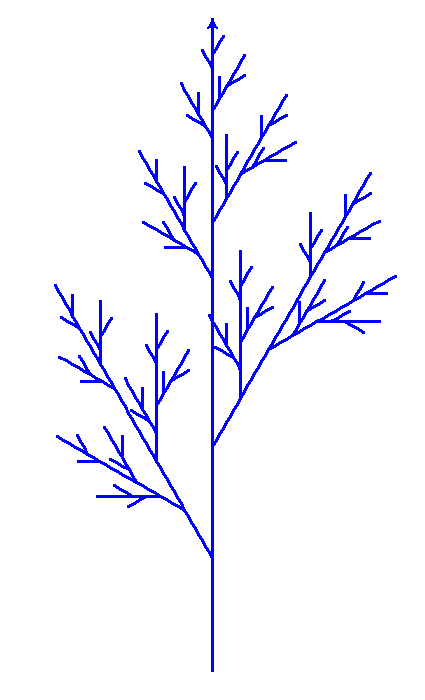
\includegraphics[scale=\myscale,scale=0.3]{screen-lsystems-14}
\end{center}

\index{L-systems}
\index{replace}
\index{turtle}


%%%%%%%%%%%%%%%%%%%%%%%%%%%%%%%%%%%%%%%%%%%%%%%%%%%%%%%%%%%%%%%%
%%%%%%%%%%%%%%%%%%%%%%%%%%%%%%%%%%%%%%%%%%%%%%%%%%%%%%%%%%%%%%%%

\begin{cours}[L-system]
An \defi{L-system} is the data of an initial word and replacement rules.
Here is an example with a starting word and only one rule: 
\mycenterline{\mot{BlArB} \qquad \mot{A} $\rightarrow$ \mot{ABA}}


The \defi{$k$-iteration} of the L-system is obtained by applying the substitution to the starting word $k$ times.
Using our example:
\begin{itemize}
  \item First iteration. The starting word is \mot{BlArB}, the rule is \mot{A} $\rightarrow$ \mot{ABA}: we replace the \mot{A} by \mot{ABA}. We get the word \mot{BlABArB}.
  
  \item Second iteration. We start from the word obtained \mot{BlABArB}, we replace the two \mot{A} by \mot{ABA}: we get the word \mot{BlABABABArB}.
  
  \item The third iteration is \mot{BlABABABABABABABArB}, etc. 

\end{itemize}

When there are two (or more) rules, they must be applied at the same time.
Here is an example of a two-rule L-system:
\mycenterline{\mot{A} \qquad \mot{A} $\rightarrow$ \mot{BlA} \qquad \mot{B} $\rightarrow$ \mot{BB}}
With our example:
\begin{itemize}
  \item First iteration. The starting word is \mot{A}, we apply the first rule \mot{A} $\rightarrow$ \mot{BlA} (the second rule does not apply, because there is no \mot{B} yet): we get the word \mot{BlA}.
  
  \item Second iteration. We start from the word obtained \mot{BlA}, we replace the \mot{A} by \mot{BlA} and at the same time the \mot{B} by \mot{BB}: we get the word \mot{BBlBlA}.
  
  \item The third iteration is \mot{BBBBlBBlBlA}, etc.  
\end{itemize}

\end{cours}


\begin{cours}[Optional argument for a function]

\index{function!optional argument}
\index{argument}

I want to program a function that draws a line of a given length, with the possibility to change the thickness of the line and the color.

One method would be to define a function by:
 \mycenterline{\ci{def draw(length, width, color):}}
 I would then call it like this:
 \mycenterline{\ci{draw(100, 5, "blue"):}} 
But since my features will, most of the time, have a thickness of $5$ and a blue color, I lose time and legibility by giving this information each time.

\medskip

With \Python{} it is possible to create optional arguments. There is a way to use optional arguments by giving the function default values:
 \mycenterline{\ci{def draw(length, width=5, color="blue"):}}
 
\begin{itemize}
  \item The command \ci{draw(100)} draws my line, and as I only specified the length, the arguments \ci{width} and \ci{color} get the default values ($5$ and blue).
  
   \item The command \ci{draw(100, width=10)} draws my line with a new thickness (the color is the default one).
   
    \item The command \ci{draw(100, color="red")} draws my line with a new color (the thickness is the default one).  
    
     \item The command \ci{draw(100, width=10, color="red")} draws my line with a new thickness and a new color.
     
     \item We can also use:
     \begin{itemize}
       \item \ci{draw(100, 10, "red")}: no need to specify the names of the arguments if you maintain the order.
       \item \ci{draw(color="red", width=10, length=100)}: if you name the arguments, then you can pass them in any order.
 
  \end{itemize}   
\end{itemize}   
\end{cours}



%%%%%%%%%%%%%%%%%%%%%%%%%%%%%%%%%%%%%%%%%%%%%%%%%%%%%%%%%%%%%%%%
% Activity 1
%%%%%%%%%%%%%%%%%%%%%%%%%%%%%%%%%%%%%%%%%%%%%%%%%%%%%%%%%%%%%%%%

\begin{activite}[Draw a word]

\objectifs{Goal: make a drawing from a \og{}word\fg{}. Each character corresponds to a turtle instruction.}

You are given a word (for example \mot{AlArAArArA}) in which each letter (read from left to right) corresponds to an instruction for \Python's turtle.

\begin{itemize}
  \item \mot{A} or \mot{B}: advance by a fixed distance (by tracing),
  \item \mot{l}: turn left, without moving forward, by a fixed angle (most often $90$ degrees),
  \item \mot{r}: turns right by a fixed angle.
\end{itemize}

The other characters do not do anything. (More commands will be added later on.)

Program a \ci{draw_lsystem(word,angle=90,scale=1)} function
which displays the drawing corresponding to the letters of a string \ci{word}. By default the angle is $90$ degrees, and the distance you move forward is $100 \times$\ci{scale}.

For example: \ci{draw_lsystem("AlArAArArA")} displays this:
\begin{center}
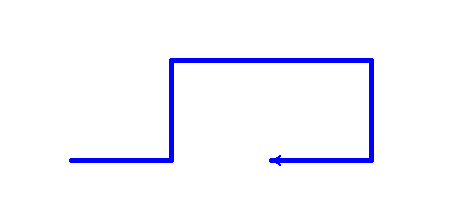
\includegraphics[scale=\myscale,scale=0.6]{screen-lsystems-1}
\end{center}

\end{activite}


%%%%%%%%%%%%%%%%%%%%%%%%%%%%%%%%%%%%%%%%%%%%%%%%%%%%%%%%%%%%%%%%
% Activity 2
%%%%%%%%%%%%%%%%%%%%%%%%%%%%%%%%%%%%%%%%%%%%%%%%%%%%%%%%%%%%%%%%

\begin{activite}[Only one rule -- Koch's snowflake]

\index{Koch's snowflake}

\objectifs{Goal: draw the Koch snowflake from a word obtained by iterations.}

\begin{center}
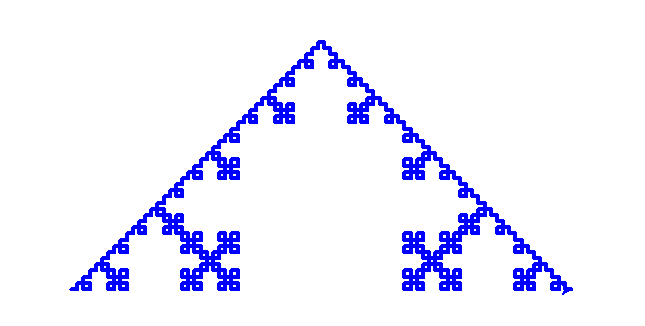
\includegraphics[scale=\myscale,scale=0.4]{screen-lsystems-2}
\end{center}

\begin{enumerate}
  \item Program a \ci{replace_1(word,letter,pattern)} function that replaces a letter with a pattern in a word. 

For example with \ci{word = "ArAAl"}, \ci{replace_1(word,"A","Al")} returns the word \ci{AlrAlAll}: each letter \mot{A} has been replaced by the pattern \mot{Al}.
 
  \item Program an \ci{iterate_lsystem_1(start,rule,k)} function
  which calculates the $k$-iteration of the L-system associated with the initial word \ci{start} according to the rule \ci{rule} which contains the pair formed by the letter and its replacement pattern.
  For example, with:
  \begin{itemize}
    \item \ci{start = "A"}
    \item \ci{rule = ("A","AlArArAlA")} i.e. \mot{A} $\rightarrow$ \mot{AlArArAlA}
    \item for \ci{k = 0}, the function returns the starting word \ci{A},
    \item for \ci{k = 1}, the function returns \ci{AlArArAlA},
    \item for \ci{k = 2}, the function returns:  
     \mycenterline{\ci{AlArArAlAlAlArArAlArAlArArAlArAlArArAlAlAlArArAlA}}
     
    \item for \ci{k = 3}, the function returns: \ci{AlArArAlAlAl...} a word of $249$ letters.
    
  \end{itemize}
  
  \item Trace the first images of the Koch's snowflake given as above by:  
  \mycenterline{start: \mot{A} \qquad rule: \mot{A} $\rightarrow$ \mot{AlArArAlA}} 
  
  
  Here are the images for $k=1$ up to $k=5$.
  For $k=1$, the word is \mot{AlArArAlA}, you can draw yourself and confirm the trace of the first image.
  
\begin{center}
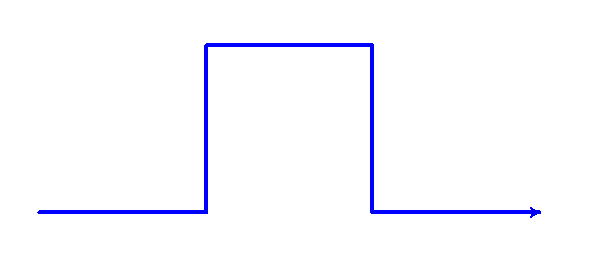
\includegraphics[scale=\myscale,scale=0.22]{screen-lsystems-3a}
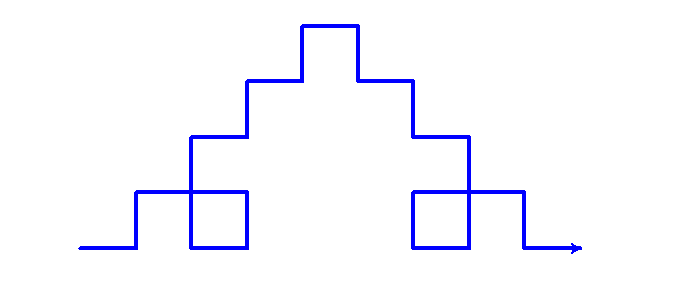
\includegraphics[scale=\myscale,scale=0.22]{screen-lsystems-3b}
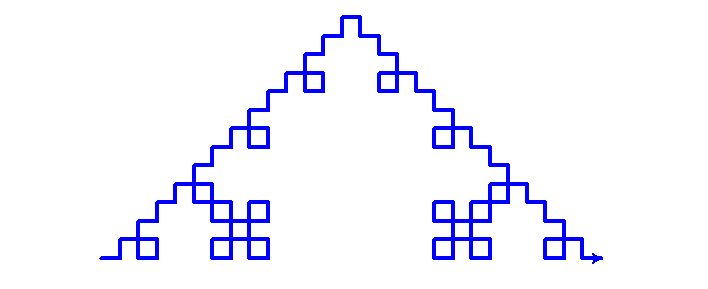
\includegraphics[scale=\myscale,scale=0.22]{screen-lsystems-3c}
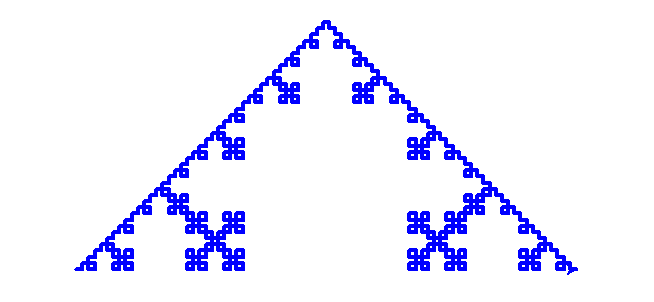
\includegraphics[scale=\myscale,scale=0.22]{screen-lsystems-3d}
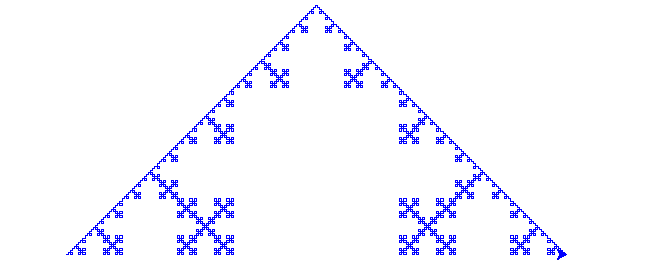
\includegraphics[scale=\myscale,scale=0.22]{screen-lsystems-3e}
\end{center}
  
	\item Trace other fractal figures from the following L-systems. For all these examples the starting word is \ci{"ArArArA"} (a square) and the rule is to be chosen among:
	
\medskip	
		
	\begin{itemize}
	  \item \ci{("A","ArAlAlAArArAlA")}
	  				 
	  \item \ci{("A","AlAArAArArAlAlAArArAlAlAAlAArA")}

	  \item \ci{("A","AArArArArAA")}
	                  
	  \item \ci{("A","AArArrArA")}

	  \item \ci{("A","AArArArArArAlA")}
	  
	  \item \ci{("A","AArAlArArAA")}
	  	                 
	  \item \ci{("A","ArAArrArA")}
	  
	  \item \ci{("A","ArAlArArA")}              
	\end{itemize}
	
\medskip	
	
\begin{center}
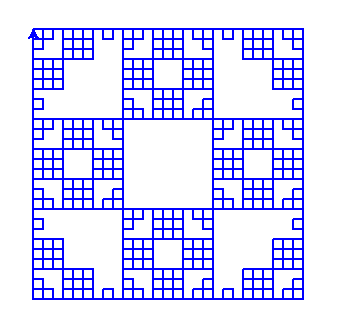
\includegraphics[scale=\myscale,scale=0.3]{screen-lsystems-4}\quad
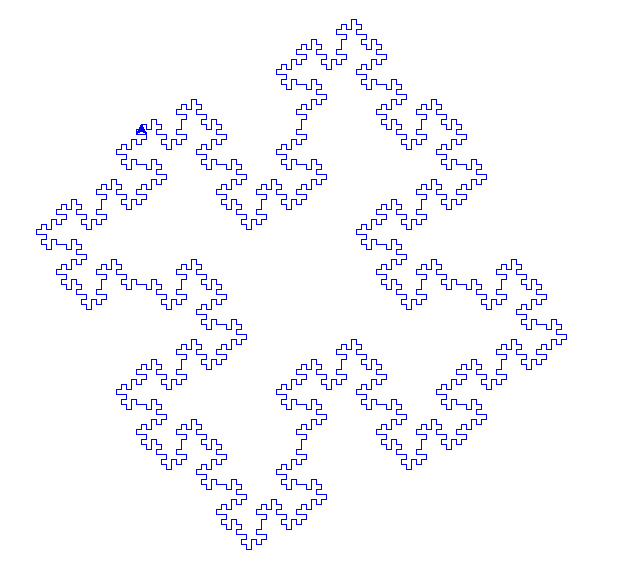
\includegraphics[scale=\myscale,scale=0.2]{screen-lsystems-5}\quad
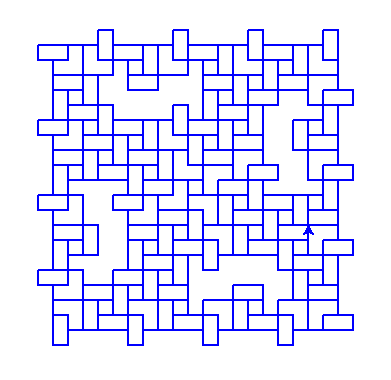
\includegraphics[scale=\myscale,scale=0.27]{screen-lsystems-6}
\end{center}


\end{enumerate}


\objectifs{Invent and trace your own L-systems!}

\end{activite}



%%%%%%%%%%%%%%%%%%%%%%%%%%%%%%%%%%%%%%%%%%%%%%%%%%%%%%%%%%%%%%%%
% Activity 3
%%%%%%%%%%%%%%%%%%%%%%%%%%%%%%%%%%%%%%%%%%%%%%%%%%%%%%%%%%%%%%%%

\begin{activite}[Two rules -- Sierpinski triangle]

\objectifs{Goal: draw more complicated L-systems by allowing two replacement rules instead of one.}

\index{Sierpinski's triangle}

\begin{center}	
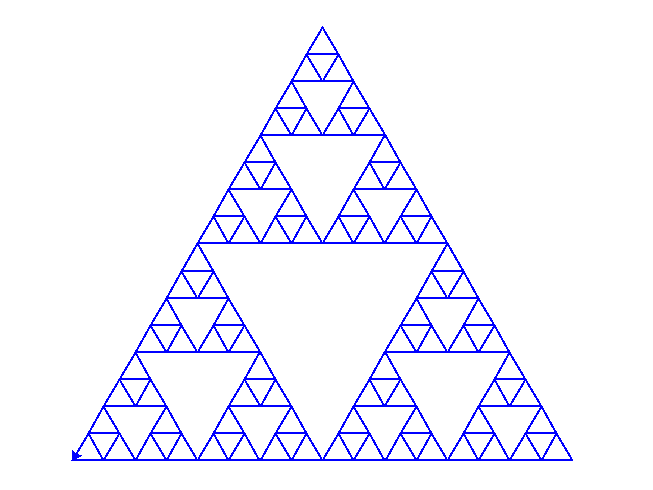
\includegraphics[scale=\myscale,scale=0.35]{screen-lsystems-7e}
\end{center}

\begin{enumerate}
  \item Program a \ci{replace_2(word,letter1,pattern1,letter2,pattern2)} function that replaces the first letter with a pattern and the second letter with another pattern. 

For example when \ci{word = "ArBlA"}, \ci{replace_2(word,"A","ABl","B","Br")} returns the word \ci{ABlrBrlABl}: each letter \mot{A} has been replaced by the pattern \mot{ABl} and at the same time each letter \mot{B} has been replaced by \mot{Br}.

\emph{Warning!} You should not get \ci{ABrlrBrlABrl}. If this is the case, it is because you used the \ci{replace_1()} function first to replace the \ci{A}, then a second time to replace the \ci{B} (but after the first replacement, new \ci{B} appeared). A new function must be programmed to avoid this. 

 
  \item Program an  \ci{iterate_lsystems_2(start,rule1,rule2,k)} function
  which calculates the $k$-iteration of the L-system associated with the initial word \ci{start}, according to the rules \ci{rule1} and \ci{rule2}.
   For example, with:
  \begin{itemize} 
    \item \ci{start = "ArBrB"}
    \item \ci{rule1 = ("A","ArBlAlBrA")} i.e. \mot{A} $\rightarrow$ \mot{ArBlAlBrA}
    \item \ci{rule2 = ("B","BB")} i.e. \mot{B} $\rightarrow$ \mot{BB}  
    \item for \ci{k = 0}, the function returns the starting word \ci{ArBrB},
    \item for \ci{k = 1}, the function returns \ci{ArBlAlBrArBBrBB},
    \item for \ci{k = 2}, the function returns:    
    \mycenterline{\ci{ArBlAlBrArBBlArBlAlBrAlBBrArBlAlBrArBBBBrBBBB}}
  \end{itemize}  

  \item Trace the first pictures of the Sierpinski triangle given as above by:  
  \mycenterline{start: \mot{ArBrB} \qquad rules: \mot{A} $\rightarrow$ \mot{ArBlAlBrA} \quad \mot{B} $\rightarrow$ \mot{BB}}
  
 The angle is $-120$ degrees. Here are the images for $k=0$ up to $k=4$.
  
\begin{center}
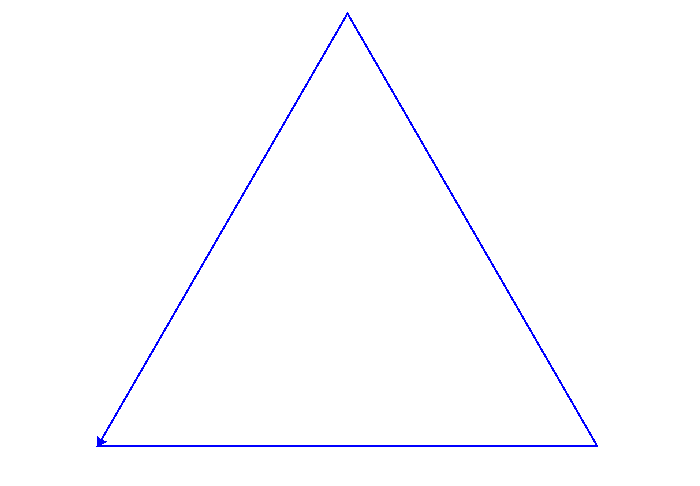
\includegraphics[scale=\myscale,scale=0.22]{screen-lsystems-7a}
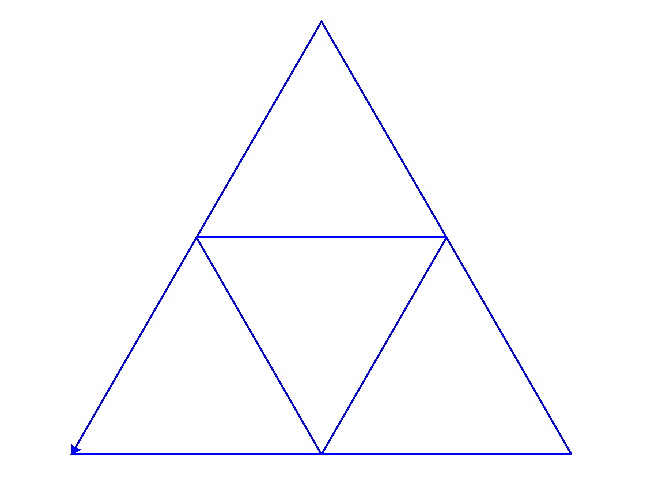
\includegraphics[scale=\myscale,scale=0.22]{screen-lsystems-7b}
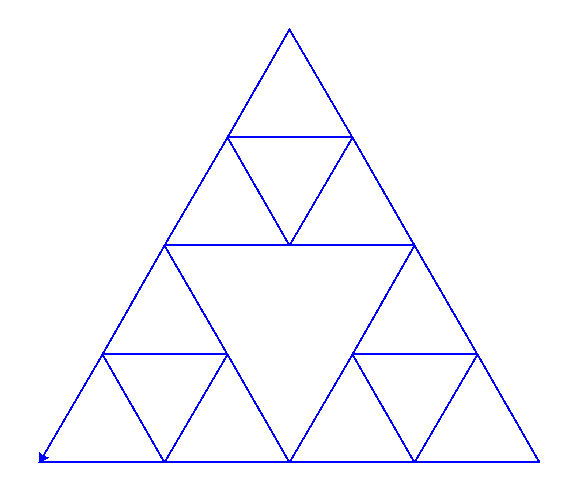
\includegraphics[scale=\myscale,scale=0.22]{screen-lsystems-7c}
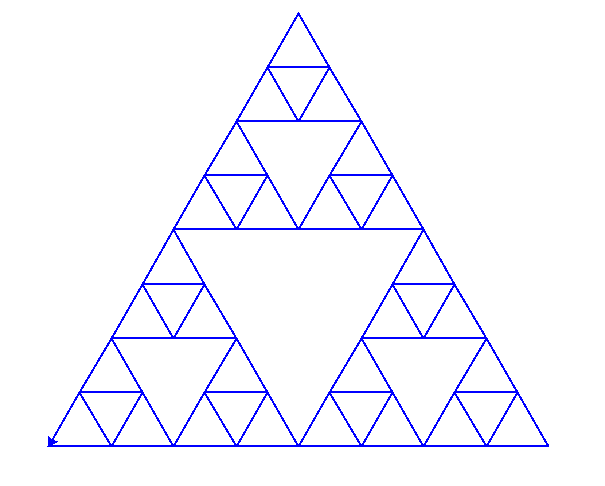
\includegraphics[scale=\myscale,scale=0.22]{screen-lsystems-7d}
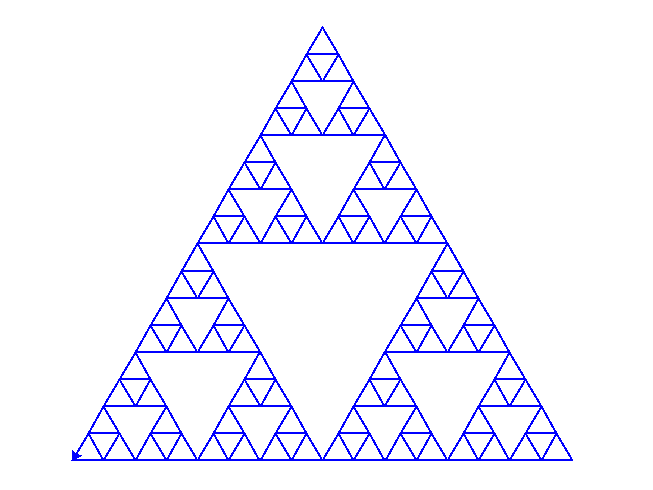
\includegraphics[scale=\myscale,scale=0.22]{screen-lsystems-7e}
\end{center}
  
	\item Trace other fractal figures from the following L-systems.
	
	\begin{itemize}
	  \item The dragon curve:
\mycenterline{\ci{
start="AX"    
rule1=("X","XlYAl")    
rule2=("Y","rAXrY")
}}

The letters \ci{X} and \ci{Y} do not correspond to an action.

	\item A variant of the Sierpinski triangle, where \ci{angle = 60}:	
\mycenterline{\ci{	
start="A"    
rule1=("A","BrArB")    
rule2=("B","AlBlA")
}}

\item The Gosper curve, where \ci{angle = 60}:
\mycenterline{\ci{start="A"}}    
\mycenterline{\ci{rule1=("A","AlBllBrArrAArBl")}}    
\mycenterline{\ci{rule2=("B","rAlBBllBlArrArB")}}
	  
	\end{itemize}
	
\begin{center}
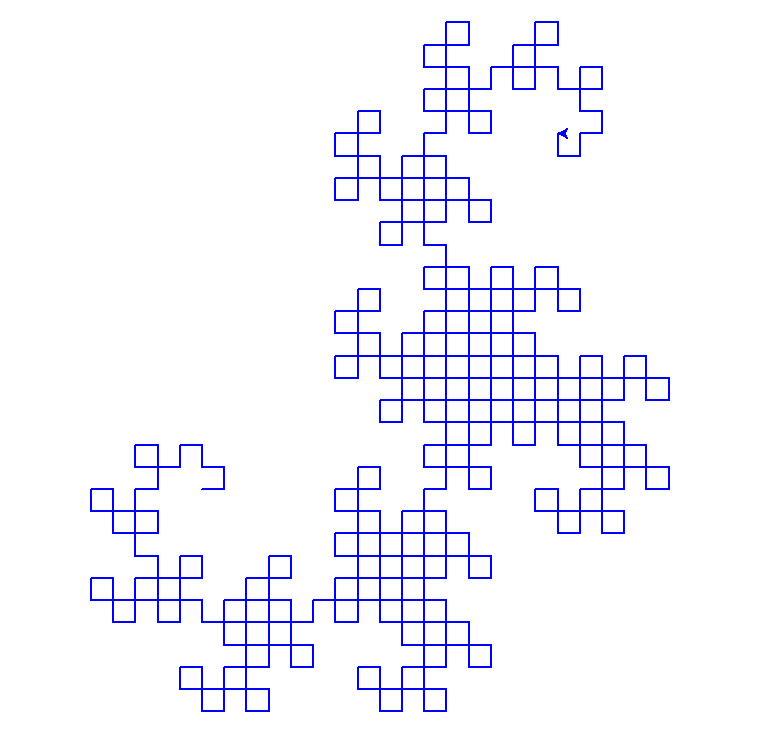
\includegraphics[scale=\myscale,scale=0.15]{screen-lsystems-8}\quad
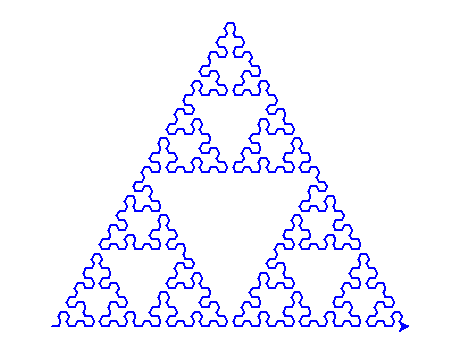
\includegraphics[scale=\myscale,scale=0.33]{screen-lsystems-9}\quad
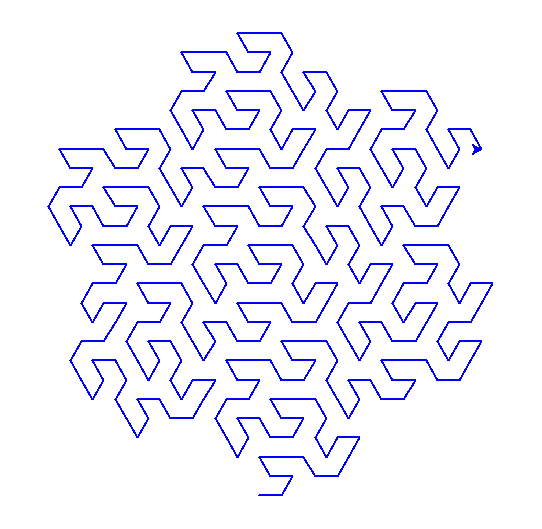
\includegraphics[scale=\myscale,scale=0.24]{screen-lsystems-10}
\end{center}


\end{enumerate}

\objectifs{Invent and trace your own L-systems with two rules!}


\end{activite}


\begin{cours}[Stacks]
A \defi{stack} is a temporary storage area. Details are in the \og{}Polish calculator -- Stacks\fg{} chapter. Here are just a few reminders.

\index{stack}

\myfigure{1}{
\tikzinput{fig-stacks}
}  

\begin{itemize}
  \item A stack is like a stack of plates; elements are placed one by one to the top of the stack; the elements are removed one by one, always from the top. It follows the \og{}last in, first out\fg{} principle.
  
  \item We model a stack using a list. 
  \item At the beginning the stack is empty: \ci{stack = []}.
  \item \textbf{Push.} We add the items to the end of the list: \ci{stack.append(element)} or \ci{stack = stack + [element]}.
  \item \textbf{Pop.} An item is removed by using the \ci{pop()}\index{pop@\ci{pop}} command:  
  \mycenterline{\ci{element = stack.pop()}}
  
  which returns the last item in the stack and removes it from the list.
  
  \item On the drawing and in the next activity, the elements of the stack are of  type $\big((x,y),\theta\big)$ that will store a state of the turtle: $(x,y)$ is the position and $\theta$ is its direction.
  
\end{itemize}

\end{cours}


%%%%%%%%%%%%%%%%%%%%%%%%%%%%%%%%%%%%%%%%%%%%%%%%%%%%%%%%%%%%%%%%
% Activity 4
%%%%%%%%%%%%%%%%%%%%%%%%%%%%%%%%%%%%%%%%%%%%%%%%%%%%%%%%%%%%%%%%

\begin{activite}[L-system, stack and turtle]

\objectifs{Goal: improve our drawings by allowing us to move forward without tracing and also by using a kind of flashback, to trace plants.}

\begin{center}
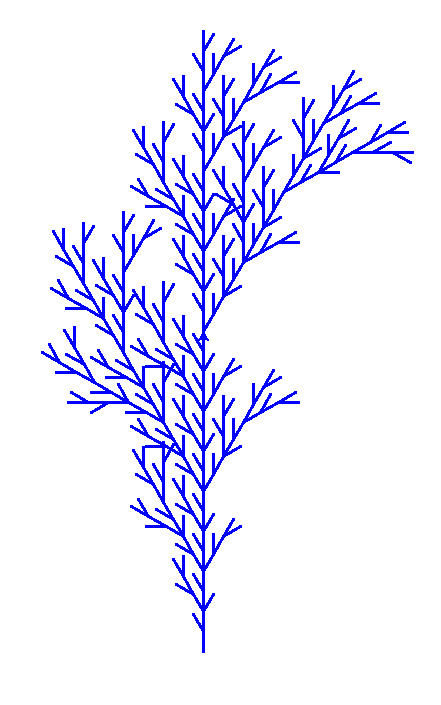
\includegraphics[scale=\myscale,scale=0.27]{screen-lsystems-17}
\end{center}

\begin{enumerate}
  \item \textbf{Forward without tracing.} 
  
  Increase the possibilities by allowing the turtle to move forward without drawing a line, when the instruction is the letter \mot{a} (in lowercase). (It is sufficient to modify the \ci{trace_lsystems()}
  function.)

Then trace the following L-system:
\begin{itemize}  
\item \ci{start = "ArArArA"}
\item \ci{rule1 = ("A","AlarAAlAlAAlAalAAralAArArAArAarAAA")}
\item \ci{rule2 = ("a","aaaaaa")}
\end{itemize}
\begin{center}
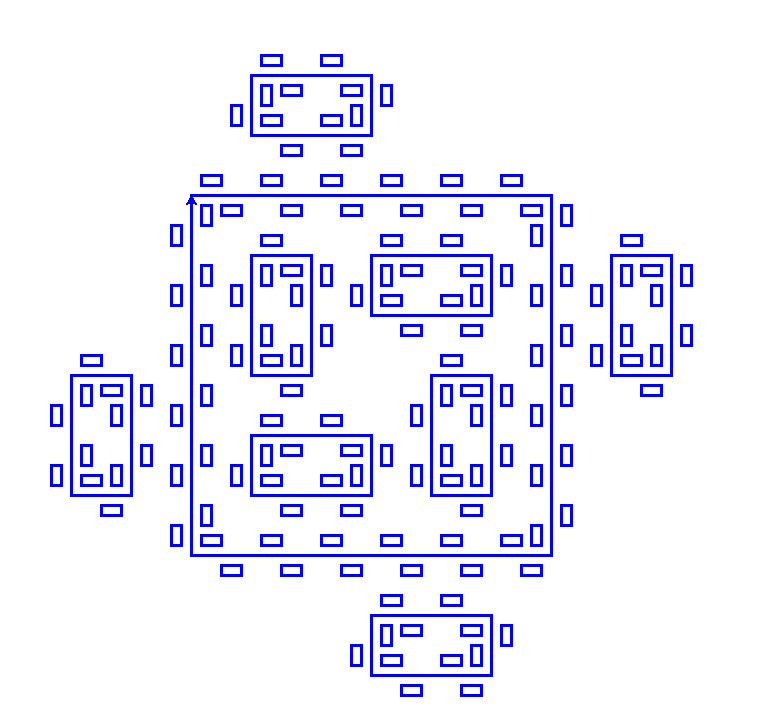
\includegraphics[scale=\myscale,scale=0.2]{screen-lsystems-11}
\end{center}  

  \item \textbf{Return back.} 
  
  We now allow square brackets in our words. For example \mot{AlA[lAAA]A[rAA]A}. When you encounter a opening bracket \og{}\mot{[}\fg{}, you store the position of the turtle, then the commands in brackets are executed as usual, when you reach the closing bracket \og{}\ci{]}\fg{} you go back to the stored position.
  
  
Let us work through the example: 
\mot{
{\color{blue}AlA}
{\color{red}[lAAA]}
{\color{green!70!black}A}
{\color{purple}[rAA]}
{\color{orange}A}
}

\myfigure{1}{
\tikzinput{fig-brackets}
}   
 
\begin{itemize}
  \item \mot{{\color{blue}AlA}}: we start from the point $O$, we move forward, we turn, we move forward.
  \item \mot{{\color{red}[lAAA]}}: we store the current position (the point $P$) and the direction; we turn, we advance three times (we trace the red segment); at the end we return the turtle to the position $P$ (without tracing and with the same direction as before).
  \item \mot{{\color{green!70!black}A}}: from $P$ we advance (green segment).
  \item \mot{{\color{purple}[rAA]}}: we store the position $Q$ and the direction, we turn and we trace the purple segment. We come back to $Q$ with the old state.
  \item \mot{{\color{orange}A}}: from $Q$ we trace the last segment.
\end{itemize}

  \medskip
  
  Here is how to draw a word containing brackets using a stack:
  \begin{itemize}
    \item At the beginning the stack is empty.
	\item We read the characters of the word one by one. The actions are the same as before.
	\item If the character is the opening bracket \og{}\mot{[}\fg{} then add the current position and direction of the turtle $\big( (x,y), \theta\big)$ to the stack. You get $\big( (x,y), \theta\big)$ by \ci{(position(), heading())}.
	
	\item If the character is the closing bracket \og{}\mot{]}\fg{} then pop 
	(i.e. read the top element of the stack and remove it). Set the position of the turtle and the angle to the read values. Use \ci{goto()} and \ci{setheading()}.
	
	\end{itemize}
	
	\item Trace the following L-systems, where the starting word and rule (or rules) are given. The angle is to be chosen between $20$ and $30$ degrees.
	
\begin{itemize}

	  \item 
\ci{"A"} \quad 
\ci{("A","A[lA]A[rA][A]")}
	  
	  \item 
\ci{"A"} \quad 
\ci{("A","A[lA]A[rA]A")}
	  
	  \item 
\ci{"A"} \quad 
\ci{("A","AAr[rAlAlA]l[lArArA]")}

	  \item 
\ci{"X"} \quad  
\ci{("X","A[lX][X]A[lX]rAX")} \quad 
\ci{("A","AA")}
	  
	\item 
\ci{"X"} \quad 
\ci{("X","A[lX]A[rX]AX")} \quad 
\ci{("A","AA")}

	\item 
\ci{"X"} \quad 
\ci{("X","Ar[[X]lX]lA[lAX]rX")} \quad 
\ci{("A","AA")}
	\end{itemize}
	
\begin{center}
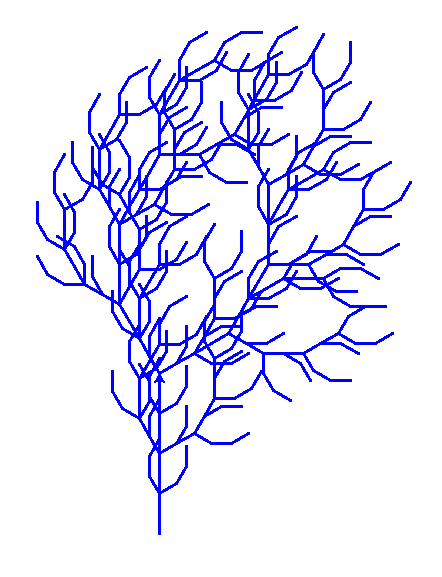
\includegraphics[scale=\myscale,scale=0.27]{screen-lsystems-15}\qquad
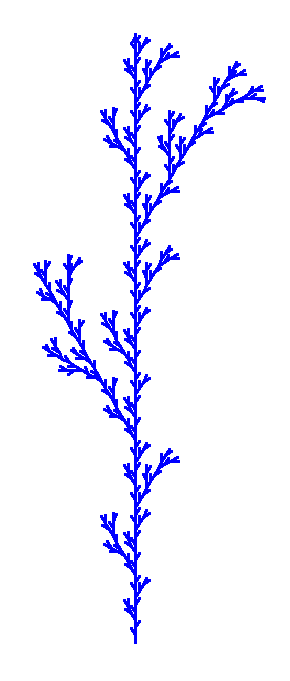
\includegraphics[scale=\myscale,scale=0.25]{screen-lsystems-16}\qquad
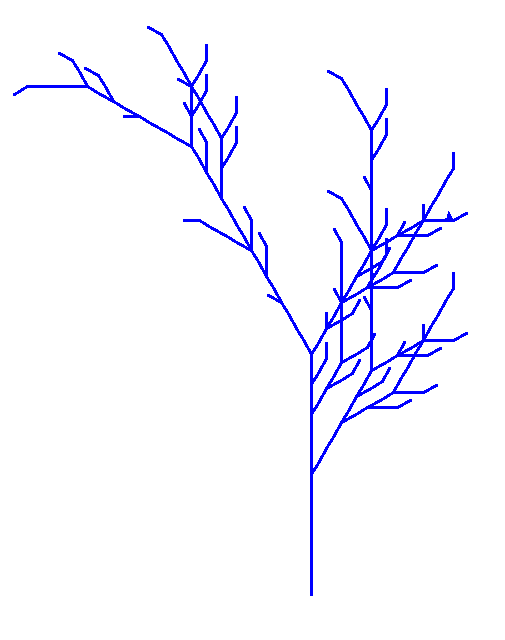
\includegraphics[scale=\myscale,scale=0.25]{screen-lsystems-12}
\end{center}
	
  
 \end{enumerate}

\objectifs{Invent your own plant!}

\end{activite}


\end{document}
